\documentclass[11pt,a4paper]{article}

\usepackage[utf8]{inputenc}
\usepackage[T1]{fontenc}
\usepackage[italian]{babel}
\usepackage{graphicx}
\usepackage{listings}
\usepackage{xcolor}
\usepackage{geometry}
\usepackage{hyperref}

\geometry{margin=2.5cm}
\graphicspath{{Progettazione/cpi/}{Progettazione/heat/}}

\lstset{
  basicstyle=\ttfamily\small,
  breaklines=true,
  frame=single,
  columns=fullflexible
}

\title{Relazione 3}
\author{Federico Becchi}
\date{\today}

\begin{document}

\maketitle

\section{Calcolo PiGreco}

L'obbiettivo del programma è calcolare il pigreco, vengono utilizzati due metodi: f1, f2.
Si sta utilizzando la funzione f2.

Esecuzione file \texttt{cpi.slurm}

\begin{lstlisting}
N=100000000

gcc cpi.c -O2 -o cpi -lm
./cpi -n $N

gcc cpi+amdahl.c -O2 -o cpi+amdahl -lm
./cpi+amdahl -n $N -s 100000
\end{lstlisting}

Il file \texttt{cpi.slurm.2510099.out} è il file di output:

\begin{lstlisting}
[federico.becchi@ui01 cpi]$ cat cpi.slurm.2510099.out
#Inter       error       time         hostname
 100000000,  1.04760645e-12,  1.01459, wn23
#Inter       error     tp       tnp     tp1+tnp        hostname
 100000000,  6.33271213e-13,  0.55609,  0.10016, 0.65625, wn23
[federico.becchi@ui01 cpi]$
\end{lstlisting}

\begin{figure}[h!]
  \centering
  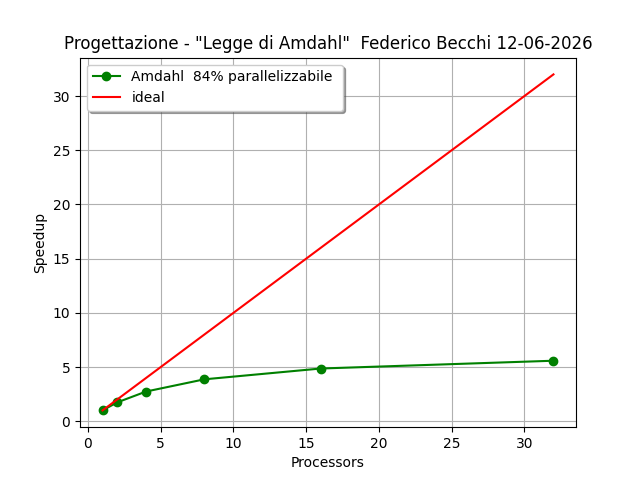
\includegraphics[width=0.7\textwidth]{../Progettazione/cpi/cpi+amdahl.png}
  \caption{../Progettazione/cpi/cpi+amdahl.png}
\end{figure}

\section{Heat}

\texttt{heat.c} vuole simulare la propagazione del calore con i bordi e il centro mantenuti a temperatura costante (1.0).

\begin{lstlisting}
gcc -O2 heat.c -o heat

./heat -d -r 20 -c 20   (numero di righe 20, numero di colonne 20)

./heat 1>heatmap.txt 2>heat.csv
\end{lstlisting}

\texttt{heatmap.txt} è la matrice finale dopo le iterazioni.

\texttt{heat.csv} è la stringa composta da:

\begin{lstlisting}
NX,NY,MAX_ITER,time, Jtime (jacobi update)
512, 512, 1000, 0.364, 0.329
\end{lstlisting}

\subsection*{heat\_scaling.slurm}

Vuole fare uno scaling test di heat, per vedere come cambiano i tempi di esecuzione all'aumentare della dimensione della matrice.

\begin{lstlisting}
(venv) [federico.becchi@ui01 heat]$ cat heat_scaling.csv
nx,  ny,  iter,  time,  jtime
512, 512, 1000, 0.379, 0.344
758, 758, 1000, 1.044, 1.018
1024, 1024, 1000, 2.737, 2.598
2048, 2048, 1000, 13.909, 12.357
\end{lstlisting}

\begin{figure}[h!]
  \centering
  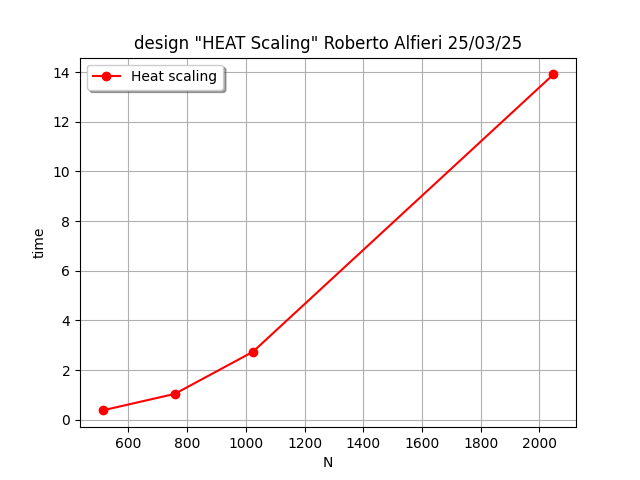
\includegraphics[width=0.7\textwidth]{../Progettazione/heat/heat_scaling.png}
  \caption{heat\_scaling.png}
\end{figure}

\begin{figure}[h!]
  \centering
  
\includegraphics[width=0.7\textwidth]{../Progettazione/heat/heatmap-animation-frame0.png}
  \caption{heatmap-animation.gif (primo frame, il PDF non supporta le GIF animate)}
\end{figure}

\subsection*{heat-pg.slurm}

\texttt{gcc -O2 -pg heat.c -o heat-pg}: si attivano i flag \texttt{-pg} per mettere le info di profiling.

\begin{lstlisting}
  %   cumulative   self              self     total
 time   seconds   seconds    calls  Ts/call  Ts/call  name
 80.41     15.70    15.70                             Jacobi_Iterator_CPU
 19.31     19.47     3.77                             Init_center
  0.46     19.56     0.09                             copy_cols
  0.31     19.62     0.06                             print_colormap
\end{lstlisting}

\section{Factorize}

Il programma fattorizza a forza bruta, ovvero genera una sequenza di numeri primi $p$ (dispari) e verifica il resto della divisione Modulo/$p$.

Esecuzione di \texttt{time} con modulo a 68 bit di cui 8 bit di address ($2^8$ blocchi disponibili) e ogni blocco ha $2^{26}$ numeri dispari da testare.

\begin{lstlisting}
sbatch factorize.slurm
\end{lstlisting}

Questo è il modulo usato: \texttt{MODULUS=B81915BC0A2222F4B}

\begin{lstlisting}
processed block 221 in 2.2 sec. with result 1
FOUND: 375C8B8B3

real	2m41.694s
user	2m41.307s
sys	0m0.002s
\end{lstlisting}

\subsection{Decomposizione del dominio}

La decomposizione del dominio è un vettore di $[1,2^{primebit}]$ numeri.
Il sorgente \texttt{factorize.c} lo scompone già in blocchi continui di dimensione $2^{block\_dim\_bit}$, il numero totale di blocchi è $2^{block\_addr\_bit}$.

Si tratta di una decomposizione a blocchi continua ove ogni blocco è un intervallo di numeri consecutivi.

Quello applicato è un bilanciamento a grana grossa in cui un numero di blocchi eseguono la ricerca del fattore. La ricerca all'interno del blocco non è prevedibile e sbilanciata.

\subsection{Legge di Amdahl applicata a questo problema}

Come parte parallelizzabile si assume la sezione di ricerca del fattore all'interno del blocco.
Come parte seriale quella antecedente all'esecuzione della ricerca e successiva al blocco.

\paragraph{Speedup ideale} Il fattore dovrebbe essere sempre nell'ultimo blocco per ottenere un incremento lineare rispetto al numero di thread/processi.

\paragraph{Speedup reale misurato} L'overhead è trascurabile nelle parti seriali, tuttavia una parallelizzazione non comporta un reale aumento delle performance a livello di tempo.

\subsection{Overhead: memoria condivisa vs distribuita}

\paragraph{Memoria Condivisa}
L'overhead si ottiene nella sincronizzazione nell'accesso alle variabili condivise $M,F$.
Invece il load balancing si può ottenere con uno scheduling dinamico, ovvero appena un thread finisce l'esecuzione del suo job può essere assegnato ad un blocco non ancora processato.

\paragraph{Memoria distribuita}
Non si pone il problema di race condition sull'accesso a $M,F$.
Si ottiene un overhead di comunicazione quando un task si ferma e notifica di aver trovato il fattore.
Questo comporta che ogni job periodicamente dovrà controllare la ricezione del messaggio di fine per poi ritornare alla ricerca del fattore.

\end{document}
